% AUTO-GENERATED from Paper 1 physics-gate ablation evidence; do not hand-edit.
\newcommand{\figPaperOneGateAblation}{%
\begin{figure*}[t]
\centering
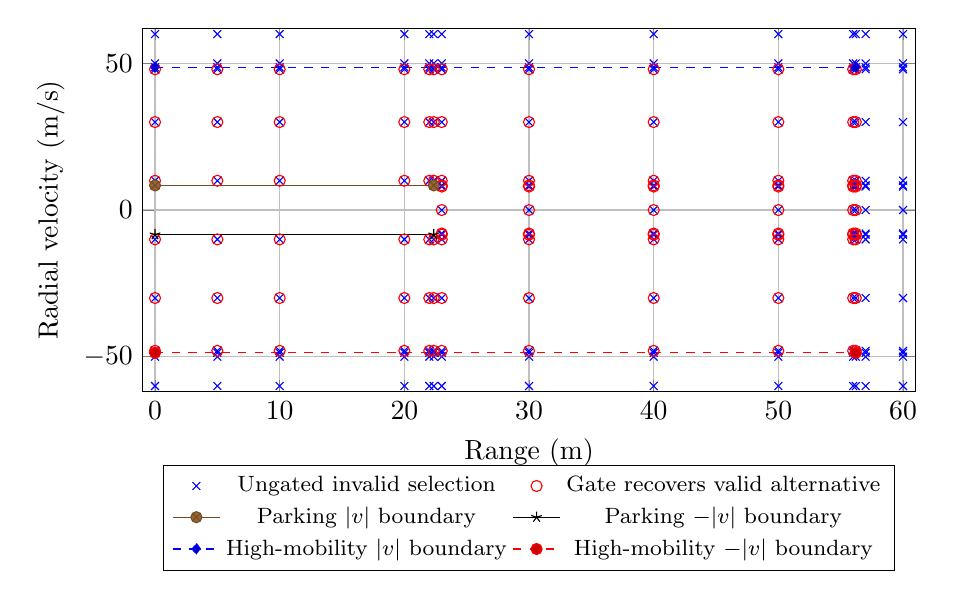
\begin{tikzpicture}
\begin{axis}[width=0.94\textwidth,height=6.2cm,xlabel={Range (m)},ylabel={Radial velocity (m/s)},xmin=-1,xmax=61,ymin=-62,ymax=62,grid=major,legend style={font=\footnotesize,at={(0.5,-0.20)},anchor=north,legend columns=2}]
\addplot+[only marks,mark=x] coordinates {(0,-60) (0,-50) (0,-48.67) (0,-48) (0,-30) (0,-10) (0,10) (0,30) (0,48) (0,48.67) (0,50) (0,60) (5,-60) (5,-50) (5,-48.67) (5,-48) (5,-30) (5,-10) (5,10) (5,30) (5,48) (5,48.67) (5,50) (5,60) (10,-60) (10,-50) (10,-48.67) (10,-48) (10,-30) (10,-10) (10,10) (10,30) (10,48) (10,48.67) (10,50) (10,60) (20,-60) (20,-50) (20,-48.67) (20,-48) (20,-30) (20,-10) (20,10) (20,30) (20,48) (20,48.67) (20,50) (20,60) (22,-60) (22,-50) (22,-48.67) (22,-48) (22,-30) (22,-10) (22,10) (22,30) (22,48) (22,48.67) (22,50) (22,60) (22.36,-60) (22.36,-50) (22.36,-48.67) (22.36,-48) (22.36,-30) (22.36,-10) (22.36,10) (22.36,30) (22.36,48) (22.36,48.67) (22.36,50) (22.36,60) (23,-60) (23,-50) (23,-48.67) (23,-48) (23,-30) (23,-10) (23,-8.41) (23,-8) (23,0) (23,8) (23,8.41) (23,10) (23,30) (23,48) (23,48.67) (23,50) (23,60) (30,-60) (30,-50) (30,-48.67) (30,-48) (30,-30) (30,-10) (30,-8.41) (30,-8) (30,0) (30,8) (30,8.41) (30,10) (30,30) (30,48) (30,48.67) (30,50) (30,60) (40,-60) (40,-50) (40,-48.67) (40,-48) (40,-30) (40,-10) (40,-8.41) (40,-8) (40,0) (40,8) (40,8.41) (40,10) (40,30) (40,48) (40,48.67) (40,50) (40,60) (50,-60) (50,-50) (50,-48.67) (50,-48) (50,-30) (50,-10) (50,-8.41) (50,-8) (50,0) (50,8) (50,8.41) (50,10) (50,30) (50,48) (50,48.67) (50,50) (50,60) (56,-60) (56,-50) (56,-48.67) (56,-48) (56,-30) (56,-10) (56,-8.41) (56,-8) (56,0) (56,8) (56,8.41) (56,10) (56,30) (56,48) (56,48.67) (56,50) (56,60) (56.21,-60) (56.21,-50) (56.21,-48.67) (56.21,-48) (56.21,-30) (56.21,-10) (56.21,-8.41) (56.21,-8) (56.21,0) (56.21,8) (56.21,8.41) (56.21,10) (56.21,30) (56.21,48) (56.21,48.67) (56.21,50) (56.21,60) (57,-60) (57,-50) (57,-48.67) (57,-48) (57,-30) (57,-10) (57,-8.41) (57,-8) (57,0) (57,8) (57,8.41) (57,10) (57,30) (57,48) (57,48.67) (57,50) (57,60) (60,-60) (60,-50) (60,-48.67) (60,-48) (60,-30) (60,-10) (60,-8.41) (60,-8) (60,0) (60,8) (60,8.41) (60,10) (60,30) (60,48) (60,48.67) (60,50) (60,60)};
\addplot+[only marks,mark=o] coordinates {(0,-48) (0,-30) (0,-10) (0,10) (0,30) (0,48) (5,-48) (5,-30) (5,-10) (5,10) (5,30) (5,48) (10,-48) (10,-30) (10,-10) (10,10) (10,30) (10,48) (20,-48) (20,-30) (20,-10) (20,10) (20,30) (20,48) (22,-48) (22,-30) (22,-10) (22,10) (22,30) (22,48) (22.36,-48) (22.36,-30) (22.36,-10) (22.36,10) (22.36,30) (22.36,48) (23,-48) (23,-30) (23,-10) (23,-8.41) (23,-8) (23,0) (23,8) (23,8.41) (23,10) (23,30) (23,48) (30,-48) (30,-30) (30,-10) (30,-8.41) (30,-8) (30,0) (30,8) (30,8.41) (30,10) (30,30) (30,48) (40,-48) (40,-30) (40,-10) (40,-8.41) (40,-8) (40,0) (40,8) (40,8.41) (40,10) (40,30) (40,48) (50,-48) (50,-30) (50,-10) (50,-8.41) (50,-8) (50,0) (50,8) (50,8.41) (50,10) (50,30) (50,48) (56,-48) (56,-30) (56,-10) (56,-8.41) (56,-8) (56,0) (56,8) (56,8.41) (56,10) (56,30) (56,48) (56.21,-48) (56.21,-30) (56.21,-10) (56.21,-8.41) (56.21,-8) (56.21,0) (56.21,8) (56.21,8.41) (56.21,10) (56.21,30) (56.21,48)};
\addplot+[domain=0:22.36,samples=2] {8.4055};
\addplot+[domain=0:22.36,samples=2] {-8.4055};
\addplot+[domain=0:56.21,samples=2,dashed] {48.6676};
\addplot+[domain=0:56.21,samples=2,dashed] {-48.6676};
\legend{Ungated invalid selection,Gate recovers valid alternative,Parking $|v|$ boundary,Parking $-|v|$ boundary,High-mobility $|v|$ boundary,High-mobility $-|v|$ boundary}
\end{axis}
\end{tikzpicture}
\caption{Boundary-aware Paper-1 ablation. Crosses mark states where the nominal ungated selector chooses a configuration outside its deterministic FMCW support; circles identify the subset for which physics gating instead exposes a valid alternative. Lines show the two profiles' unambiguous-velocity boundaries; range support is additionally enforced in the machine-readable evidence. This is deterministic analytical/simulation-model evidence, not a hardware measurement.}
\label{fig:p1gateablation}
\end{figure*}%
}
